\documentclass[tikz,border=10mm]{standalone}
\usetikzlibrary{calc,intersections}
\begin{document}
	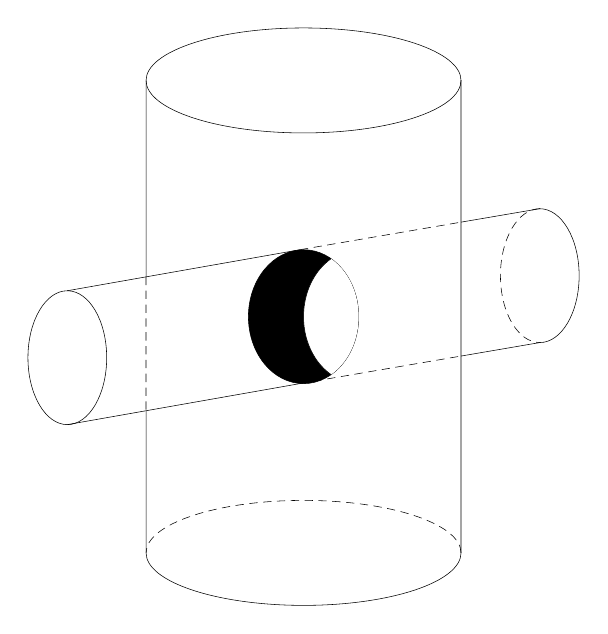
\begin{tikzpicture}[line join=round,very thin]
		\def\r{2}
		\def\h{3}
		\pgfmathsetmacro\g{10}
		\pgfmathsetmacro\y{1.5*\r *sin(\g)}
		\pgfmathsetmacro\rm{0.5*\r}
		\pgfmathsetmacro\b{.85*\rm}
		\path(-\r,\h)coordinate(C) (-\r,-\h)coordinate(C') (\r,\h)coordinate(D) (\r,-\h)coordinate(D');
		\begin{scope}[rotate=\g]
			\draw [rotate=-\g]
			(-1.5*\r,-\b-\y)coordinate(F) arc(-90:90:{0.5*\rm} and {\b})coordinate(E)arc(90:270:{0.5*\rm} and {\b})
			(1.5*\r,\b+\y)coordinate(H) arc(90:-90: {0.5*\rm} and {\b})coordinate(G);
			\draw [rotate=-\g,densely dashed](H) arc(90:270: {0.5*\rm} and {\b});
			\draw(E)--++(1.5*\r,0) coordinate(A)(F)--++(1.5*\r,0) coordinate(B);
			\path(intersection of A--E and C--C')coordinate(E')
			(intersection of B--F and C--C')coordinate(F');
			\draw [densely dashed] (E')--(F');
			\path(intersection of A--H and D--D')coordinate(H');
			\path(intersection of B--G and D--D')coordinate(G');
			\draw [densely dashed] (A)--(H')(B)--(G');
			\draw (H)--(H')(G)--(G');
			\draw[rotate=-\g,fill=black](0,0) ellipse ({.7*\rm} and {\b});
			\clip[rotate=-\g] (0,0) ellipse ({.7*\rm} and {\b});
			\draw[rotate=-\g,fill=white] (.7*\rm,0) ellipse ({.7*\rm} and {\b});
		\end{scope}
		\draw(C)--(E')(C')--(F')(D)--(D');
		\draw[densely dashed] (D') arc (0:180:{\r} and {\r/3});
		\draw (D') arc (0:-180:{\r} and {\r/3}) (D) arc (0:360:{\r} and {\r/3});
	\end{tikzpicture}
\end{document}